\documentclass{homeworg}

\title{Theoretical exercise 3}
\author{Håvard Godal}
\begin{document}
\maketitle

\problem

Assume that the underlying a priori probabilities and class conditional 
probability density functions from problem 2, exercise 2 is unknown. 
However, we have access to measurements so that we have the following samples 
from the two categories:

\begin{equation}
    \chi_1 = \left\{\binom{2}{6}, \binom{3}{4}, \binom{3}{8}, \binom{4}{6}\right\}
\end{equation}
and
\begin{equation}
    \chi_2 = \left\{\binom{1}{-2}, \binom{2.7}{-4}, \binom{3.3}{0}, \binom{5}{-2}\right\}
\end{equation}

\bigskip
\newpage
\textbf{a)} - Assuming a Gaussian distribution, use a parametric approach to formulate the Bayes classifier. Apply the maximum-likelihood (ML) method to estimate the required functions.
\smallskip

Finding $\bm{\mu}$ and $\bm{\Sigma}$ for each class $\omega_1$ and $\omega_2$ by using using the maximum-likelihood-estimators for a multivariate gaussian distribuion:

For $\bm{\mu}_i$:
\begin{equation}
    \begin{aligned}
        \bm{\hat{\mu}}_1 &= \frac{1}{n}\sum_{i=1}^n \bm{x}_i
        \\
        &= \frac{1}{4}\left[ \binom{2}{6} + \binom{3}{4} + \binom{3}{8} + \binom{4}{6} \right]
        \\
        &= \binom{3}{6}
    \end{aligned}
\end{equation}

\begin{equation}
    \begin{aligned}
        \bm{\hat{\mu}}_2 &= \frac{1}{n}\sum_{i=1}^n \bm{x}_i
        \\
        &= \frac{1}{4}\left[ \binom{1}{-2} + \binom{2.7}{-4} + \binom{3.3}{0} + \binom{5}{-2} \right]
        \\
        &= \binom{3}{-2}
    \end{aligned}
\end{equation}

For $\bm{\Sigma}_i$:
\begin{equation}
    \begin{aligned}
        \bm{\hat{\Sigma}}_1 &= \frac{1}{n}\sum_{i=1}^n(\bm{x}_i - \bm{\hat{\mu}}_1)(\bm{x}_i - \bm{\hat{\mu}}_1)^T
        \\
        &=\frac{1}{4}\left[
            \begin{pmatrix}-1\\0\end{pmatrix}\begin{pmatrix} -1&0 \end{pmatrix} +
            \begin{pmatrix}0\\-2\end{pmatrix}\begin{pmatrix} 0&-2 \end{pmatrix} +
            \begin{pmatrix}0\\2\end{pmatrix}\begin{pmatrix} 0&2 \end{pmatrix} +
            \begin{pmatrix}1\\0\end{pmatrix}\begin{pmatrix} 1&0 \end{pmatrix}
        \right]
        \\
        &=\frac{1}{4}\left[
            \begin{pmatrix}1&0\\0&0\end{pmatrix} + 
            \begin{pmatrix}0&0\\0&4\end{pmatrix} + 
            \begin{pmatrix}0&0\\0&4\end{pmatrix} + 
            \begin{pmatrix}1&0\\0&0\end{pmatrix}
        \right]
        \\
        &=\frac{1}{4}\begin{pmatrix}2&0\\0&8\end{pmatrix}
        \\
        &=\begin{pmatrix}\frac{1}{2}&0\\0&2\end{pmatrix}
    \end{aligned}
\end{equation}

\begin{equation}
    \begin{aligned}
        \bm{\hat{\Sigma}}_2 &= \frac{1}{n}\sum_{i=1}^n(\bm{x}_i - \bm{\hat{\mu}}_1)(\bm{x}_i - \bm{\hat{\mu}}_1)^T
        \\
        &=\frac{1}{4}\left[
            \begin{pmatrix}-2\\0\end{pmatrix}\begin{pmatrix} -2&0 \end{pmatrix} +
            \begin{pmatrix}-0.3\\-2\end{pmatrix}\begin{pmatrix} -0.3&-2 \end{pmatrix} +
            \begin{pmatrix}0.3\\2\end{pmatrix}\begin{pmatrix} 0.3&2 \end{pmatrix} +
            \begin{pmatrix}2\\0\end{pmatrix}\begin{pmatrix} 2&0 \end{pmatrix}
        \right]
        \\
        &=\frac{1}{4}\left[
            \begin{pmatrix}4&0\\0&0\end{pmatrix} + 
            \begin{pmatrix}0.09&0.6\\0.6&4\end{pmatrix} + 
            \begin{pmatrix}0.09&0.6\\0.6&4\end{pmatrix} + 
            \begin{pmatrix}4&0\\0&0\end{pmatrix}
        \right]
        \\
        &=\frac{1}{4}\begin{pmatrix}8.18&1.2\\1.2&8\end{pmatrix}
        \\
        &=\begin{pmatrix}2.045&0.3\\0.3&2\end{pmatrix}
    \end{aligned}
\end{equation}

Based on the number of observations of each class, the following priors are determined:
\begin{equation}
    P(\omega_1) = \frac{4}{8} = \frac{1}{2}
\end{equation}

\begin{equation}
    P(\omega_2) = \frac{4}{8} = \frac{1}{2}
\end{equation}

Bayes decision rule is as follows:
\begin{equation}
    \text{Decide }
    \left\{\begin{matrix*}[l]
        \omega_1& \text{if } P(\omega_1|\bm{x}) > P(\omega_2|\bm{x})\\ 
        \omega_2& \text{otherwise} 
    \end{matrix*}\right.
\end{equation}

Using the same procedure as in \textit{Exercise 2, problem 2} to calculate the discriminant functions $g_1(\bm{x})$ and $g_2(\bm{x})$:
\begin{equation}
    g_i(\bm{x}) = \bm{x}^T\bm{\Theta}_i\bm{x}+\bm{\theta}_i^T\bm{x}+\theta_{i0}
\end{equation}
where:
\begin{equation}
    \begin{aligned}
        \bm{\Theta}_i &= -\frac{1}{2}\Sigma_i^{-1} \\
        \bm{\theta}_i &= \Sigma_i^{-1}\bm{\mu}_i \\
        \theta_{i0} &= -\frac{1}{2}\mu_i^T\Sigma_i^{-1}\mu_i-\frac{1}{2}\ln\abs{\Sigma_i}+\ln(P(\omega_i))
    \end{aligned}
\end{equation}

Solving for $g_1(\bm{x})$:

\begin{equation}
    \begin{aligned}
        \bm{\Theta}_1 &= -\frac{1}{2}
        \begin{bmatrix}
            2 & 0 \\
            0 & 1/2
        \end{bmatrix}
        \\ &=
        \begin{bmatrix}
            -1 & 0 \\
            0 & -1/4
        \end{bmatrix}
    \end{aligned}
\end{equation}

\begin{equation}
    \begin{aligned}
        \bm{\theta}_1 &=
        \begin{bmatrix}
            2 & 0 \\
            0 & 1/2
        \end{bmatrix}
        \begin{bmatrix}
            3 \\ 6
        \end{bmatrix}
        \\ &=
        \begin{bmatrix}
            6 \\
            3
        \end{bmatrix}
    \end{aligned}
\end{equation}

\begin{equation}
    \begin{aligned}
        {\theta}_{10} &=
        -\frac{1}{2}
        \begin{bmatrix}
            3 & 6
        \end{bmatrix}
        \begin{bmatrix}
            2 & 0 \\ 0 & 1/2
        \end{bmatrix}
        \begin{bmatrix}
            3 \\ 6
        \end{bmatrix}
        -\frac{1}{2}\ln(1/2*2-0*0)+\ln(1/2)
        \\ &= - 18.69314
    \end{aligned}
\end{equation}

\begin{equation}
    \begin{aligned}
        g_1(\bm{x}) &=
        \begin{bmatrix}
            x_1 & x_2
        \end{bmatrix}
        \begin{bmatrix}
            -1 & 0 \\
            0 & -1/4
        \end{bmatrix}
        \begin{bmatrix}
            x_1 \\ x_2
        \end{bmatrix} + 
        \begin{bmatrix}
            6 & 3
        \end{bmatrix}
        \begin{bmatrix}
            x_1 \\ x_2
        \end{bmatrix} - 18.69314
        \\ &=
        -x_1^2-\frac{1}{4}x_2^2+6x_1+3x_2 - 18.69314
    \end{aligned}
\end{equation}

\newpage
Solving for $g_2(\bm{x})$:

\begin{equation}
    \begin{aligned}
        \bm{\Theta}_2 &= -\frac{1}{2}
        \begin{bmatrix}
            0.5 & -0.075 \\
            -0.075 & 0.51125
        \end{bmatrix}
        \\ &=
        \begin{bmatrix}
            -0.25 & 0.0375 \\
            0.0375 & -0.255625
        \end{bmatrix}
    \end{aligned}
\end{equation}

\begin{equation}
    \begin{aligned}
        \bm{\theta}_2 &=
        \begin{bmatrix}
            0.5 & -0.075 \\
            -0.075 & 0.51125
        \end{bmatrix}
        \begin{bmatrix}
            3 \\ -2
        \end{bmatrix}
        \\ &=
        \begin{bmatrix}
            1.65 \\
            -1.2475
        \end{bmatrix}
    \end{aligned}
\end{equation}

\begin{equation}
    \begin{aligned}
        {\theta}_{20} &=
        -\frac{1}{2}
        \begin{bmatrix}
            3 & -2
        \end{bmatrix}
        \begin{bmatrix}
            0.5 & -0.075 \\
            -0.075 & 0.51125
        \end{bmatrix}
        \begin{bmatrix}
            3 \\ -2
        \end{bmatrix}
        -\frac{1}{2}\ln(2.045*2-0.3*0.3)+\ln(1/2)
        \\ &= -5.11379
    \end{aligned}
\end{equation}

\begin{equation}
    \begin{aligned}
        g_2(\bm{x}) &=
        \begin{bmatrix}
            x_1 & x_2
        \end{bmatrix}
        \begin{bmatrix}
            -0.25 & 0.0375 \\
            0.0375 & -0.255625
        \end{bmatrix}
        \begin{bmatrix}
            x_1 \\ x_2
        \end{bmatrix} + 
        \begin{bmatrix}
            1.65 &
            -1.2475
        \end{bmatrix}
        \begin{bmatrix}
            x_1 \\ x_2
        \end{bmatrix} -5.11379
        \\ &=
        -0.25x_1^2-0.255625x_2^2+0.075x_1x_2+1.65x_1-1.2475x_2-5.11379
    \end{aligned}
\end{equation}

The decision border occurs when $g_1(\bm{x}) = g_2(\bm{x})$
\begin{equation}
    \begin{aligned}
        g_1(\bm{x}) &= g_2(\bm{x}) \\
        -x_1^2-0.25x_2^2+6x_1+3x_2 - 18.69314\\ &= \\-0.25x_1^2-0.255625x_2^2+0.075x_1x_2+1.65x_1-1.2475x_2-5.11379
        \\
        -0.75x_1^2 + 0.005625x_2^2 + 4.25x_1+4.248x_2-0.075x_1x_2 -13.57935
        &= 0
    \end{aligned}
\end{equation}
Using Symbolab to solve for $x_2$:
\begin{equation}
    x_2 = \frac{-4.248+0.075x_1 \pm \sqrt{0.0225x_1^2-0.732825x_1+18.35103}}{0.01125}
\end{equation}
One of the solutions, $\cdots -\sqrt{\cdots}$, only provides values of around $-600$, which clearly does not conform with the relevant decision boundary. Therefore:
\begin{equation}
    x_2 = \frac{-4.248+0.075x_1 + \sqrt{0.0225x_1^2-0.732825x_1+18.35103}}{0.01125}
\end{equation}


\bigskip
\newpage
\textbf{b)} - Evaluate the decision border. How are the estimated density function oriented in relation to the true density functions?
\smallskip
\bigskip

\begin{figure}[H]
    \centering
        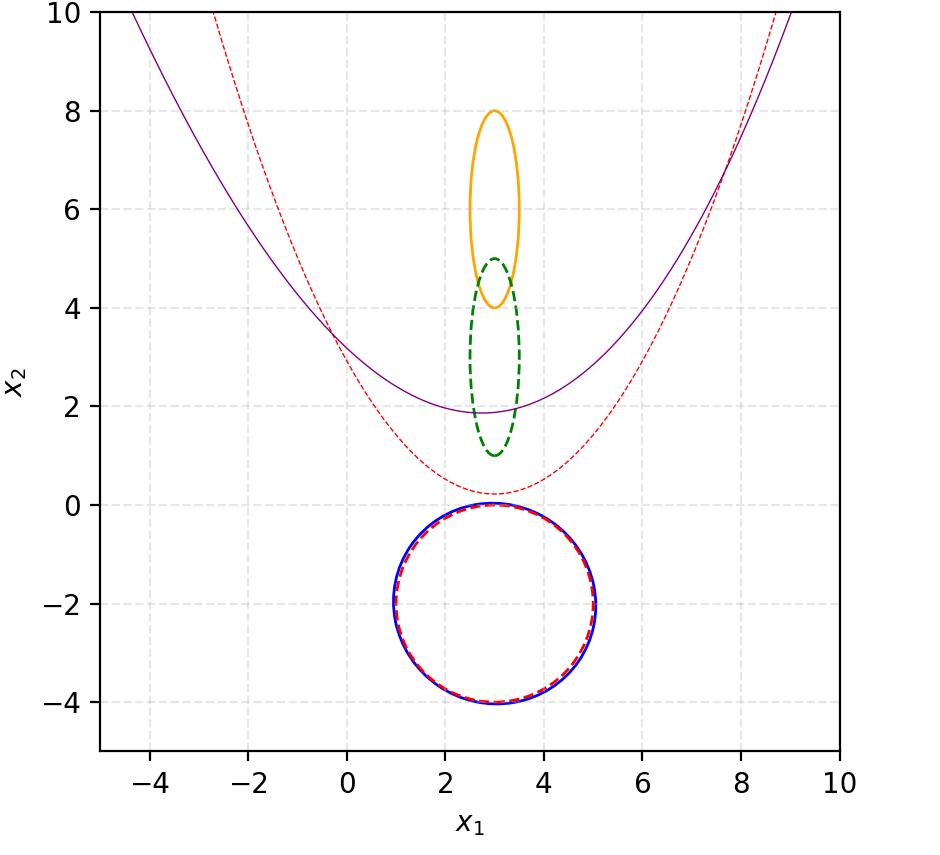
\includegraphics[scale=1]{bivariategaussian.png}
    \caption{Bivariate gaussian distributions}
\end{figure}

In \textit{Figure 1}, the dotted lines represents the true density functions and the true decision border found in \textit{Exercise 2}. 
The solid lines represent the density functions and the decision border created from the given data points.

The density of class $\omega_1$, represented with an orange ellipse from the eigenvectors, is skewed. As a result, the decision boundary is therefore also skewed.

Also, note that the new decision boundary is not symmetric around the density functions anymore.


\bigskip
\textbf{c)} - How can the decision border correspond better to the true decision border.
\smallskip
\bigskip

The best way to make the new decision border correspond better to the true decision border is to collect more data points. 

To better illustrate this, imagine throwing two dices and counting the number of eyes each time. If we take the average number of eyes from 4 throws, the difference between each turn will be great.
On the other hand, if we were to throw the two dices $1000000$ times, it would be clear that the probability density function of getting a certain amount of eyes on the dices have a Gaussian distribution.
The same goes for this exercise. More data equals a better estimation of the true value/distribution.


\problem
Using the data set from the previous problem, 
classify the feature vector $x = \begin{pmatrix}2.5&2.0\end{pmatrix}^T$.
Use the following classifiers:

\bigskip
\textbf{a)} - The Bayes classifier form \textit{Problem 1}.
\smallskip
\bigskip

\begin{equation}
    g_1(\bm{x}) = -x_1^2-\frac{1}{4}x_2^2+6x_1+3x_2 - 18.69314
\end{equation}

\begin{equation}
    \begin{aligned}
        g_1\binom{2.5}{2.0} &= -2.5^2-\frac{1}{4}2.0^2+6*2.5+3*2.0 - 18.69314
        \\
        &= -4.94314 
    \end{aligned}
\end{equation}

\begin{equation}
    g_2(\bm{x}) = -0.25x_1^2-0.255625x_2^2+0.075x_1x_2+1.65x_1-1.2475x_2-5.11379
\end{equation}
\begin{equation}
    \begin{aligned}
        g_2\binom{2.5}{2.0} &= -0.25*2.5^2-0.255625*2.0^2+0.075*2.5*2.0+1.65*2.5-1.2475*2.0-5.11379
        \\
        &= -5.69375
    \end{aligned}
\end{equation}

Because $g_1(\bm{x}) > g_2(\bm{x})$, $\bm{x}$ is classified to belong to class $\omega_1$.

\bigskip
\textbf{b)} - A Parzen-window classifier. Use a gaussian window function so that:
\begin{equation}
    p_n(\bm{x}) = \frac{1}{N}\sum_{i=1}^N\frac{1}{V_N}\phi(\bm{u})
\end{equation}
where $V_N = h_N^l$, 
\begin{equation}
    \phi(\bm{u}) = \frac{1}{(2\pi)^\frac{d}{2}\abs{\bm{I}}^\frac{1}{2}}*e^{-\frac{1}{2}(\bm{u})^T\bm{I}^{-1}(\bm{u})}
\end{equation}
with $\bm{u} = \frac{x-x_i}{h_N}$, $h_N = \frac{h_1}{\sqrt{N}}$, and $h_1 = 0.5$ 
\smallskip
\bigskip

The gaussian window function corresponds to $\sim\mathcal{N}\left(\underline{x}, h_N^2I\right)$.

$N = 4$ for both $\omega_1$ and $\omega_2$, which results in $h_N = \frac{0.5}{\sqrt{4}} = 0.25$, and $\bm{u} = \frac{x-x_i}{0.25}$.

As we are working with two dimensions, $l = d = 2$.

\medskip

As in the last subtask, the discriminant function $g_i(\bm{x}) = P(\omega_i)p_i(\bm{x}|\omega_i)$.

\begin{equation}
    \begin{aligned}
        p_n(\bm{x}) &= \frac{1}{N}\sum_{i=1}^N\frac{1}{V_N}\phi(\bm{u})
        \\
        &= \frac{1}{4}\sum_{i=1}^N\frac{1}{h_N^2}\frac{1}{(2\pi)^\frac{2}{2}\abs{\bm{I}}^\frac{1}{2}}*e^{-\frac{1}{2}(\bm{u})^T\bm{I}^{-1}(\bm{u})}
        \\
        &= \frac{1}{8\pi h_N^2}\sum_{i=1}^Ne^{-\frac{1}{2}(\frac{x-x_i}{0.25})^T\bm{I}^{-1}(\frac{x-x_i}{0.25})}
        \\
        &= \frac{1}{8\pi h_N^2}\sum_{i=1}^Ne^{-8(x-x_i)^T(x-x_i)}
        \\
        &= \frac{2}{\pi}\sum_{i=1}^Ne^{-8(x-x_i)^T(x-x_i)}
    \end{aligned}
\end{equation}

Solving for $\omega_1$:
\begin{equation}
    \begin{aligned}
        g_1(\bm{x}) &= P(\omega_1)p_n(\bm{x}|\omega_1)
        \\
        &= \frac{1}{2}\frac{2}{\pi}\sum_{i=1}^Ne^{-8(x-x_i)^T(x-x_i)}
        \\
        &= \frac{1}{\pi}\left[
        e^{-8\left(\left(2.5-2.0\right)^2 + \left(2.0-6.0\right)^2\right)} +
        e^{-8\left(\left(2.5-3.0\right)^2 + \left(2.0-4.0\right)^2\right)} +
        \cdots +
        e^{-8\left(\left(2.5-4.0\right)^2 + \left(2.0-6.0\right)^2\right)}
        \right]
        \\
        &= \frac{1}{\pi}\left[
        e^{-130}+e^{-34}+e^{-290}+e^{-146}
        \right]
        \\
        &= 5.45554E-16
    \end{aligned}
\end{equation}

Solving for $\omega_2$:
\begin{equation}
    \begin{aligned}
        g_2(\bm{x}) &= P(\omega_2)p_n(\bm{x}|\omega_2)
        \\
        &= \frac{1}{2}\frac{2}{\pi}\sum_{i=1}^Ne^{-8(x-x_i)^T(x-x_i)}
        \\
        &= \frac{1}{\pi}\left[
        e^{-8\left(\left(2.5-1.0\right)^2 + \left(2.0+2.0\right)^2\right)} +
        e^{-8\left(\left(2.5-2.7\right)^2 + \left(2.0+4.0\right)^2\right)} +
        \cdots +
        e^{-8\left(\left(2.5-5.0\right)^2 + \left(2.0+2.0\right)^2\right)}
        \right]
        \\
        &= \frac{1}{\pi}\left[
        e^{-146}+e^{-288.32}+e^{-37.12}+e^{-178}
        \right]
        \\
        &= 2.40901E-17
    \end{aligned}
\end{equation}

Because $g_1(\bm{x}) > g_2(\bm{x})$, $\bm{x}$ is classified to belong to class $\omega_1$.


\bigskip
\newpage
\textbf{c)} - A Parzen-window classifier as in the previous subtask, but with $h_1 = 5$. Compare the results and explain the change.
\smallskip
\bigskip

Changing $h_1$ from $0.5$ to $5$ results in the following changes:

$h_N = \frac{5}{\sqrt{4}} = 2.5$, and $\bm{u} = \frac{x-x_i}{2.5}$.

The computation is done the same way as the previous subtask.

\begin{equation}
    \begin{aligned}
        p_n(\bm{x}) &= \frac{1}{N}\sum_{i=1}^N\frac{1}{V_N}\phi(\bm{u})
        \\
        &= \frac{1}{4}\sum_{i=1}^N\frac{1}{h_N^2}\frac{1}{(2\pi)^\frac{2}{2}\abs{\bm{I}}^\frac{1}{2}}*e^{-\frac{1}{2}(\bm{u})^T\bm{I}^{-1}(\bm{u})}
        \\
        &= \frac{1}{8\pi h_N^2}\sum_{i=1}^Ne^{-\frac{1}{2}(\frac{x-x_i}{2.5})^T\bm{I}^{-1}(\frac{x-x_i}{2.5})}
        \\
        &= \frac{1}{8\pi h_N^2}\sum_{i=1}^Ne^{-0.08(x-x_i)^T(x-x_i)}
        \\
        &= \frac{0.02}{\pi}\sum_{i=1}^Ne^{-0.08(x-x_i)^T(x-x_i)}
    \end{aligned}
\end{equation}

Solving for $\omega_1$:
\begin{equation}
    \begin{aligned}
        g_1(\bm{x}) &= P(\omega_1)p_n(\bm{x}|\omega_1)
        \\
        &= \frac{1}{2}\frac{0.02}{\pi}\sum_{i=1}^Ne^{-0.08(x-x_i)^T(x-x_i)}
        \\
        &= \frac{0.01}{\pi}\left[
        e^{-1.30}+e^{-0.34}+e^{-2.90}+e^{-1.46}
        \right]
        \\
        &= 4.04750E-3
    \end{aligned}
\end{equation}

Solving for $\omega_2$:
\begin{equation}
    \begin{aligned}
        g_2(\bm{x}) &= P(\omega_2)p_n(\bm{x}|\omega_2)
        \\
        &= \frac{1}{2}\frac{0.02}{\pi}\sum_{i=1}^Ne^{-0.08(x-x_i)^T(x-x_i)}
        \\
        &= \frac{0.01}{\pi}\left[
        e^{-1.46}+e^{-2.8832}+e^{-0.3712}+e^{-1.78}
        \right]
        \\
        &= 3.65016E-3
    \end{aligned}
\end{equation}

Because $g_1(\bm{x}) > g_2(\bm{x})$, $\bm{x}$ is classified to belong to class $\omega_1$.

Increasing the value of $h_1$ from $0.5$ to $5$ results in a "smoother" probability density function.
This also means that the variance is increased. This is reflected in the answer, as the discriminant functions almost have the same value.
The $h$ parameter (also called the smoothing parameter) should most of the time be as small as the data will allow.
Setting $h = 50$ would result in $g_1(\bm{x}) < g_2(\bm{x})$, which justifies the claim.

\bigskip
\newpage
\textbf{d)} - A $_kN$-nearest neighbourhood classifier where $k_N = 1$.
\smallskip
\bigskip

From the lecture notes, we have that:
\begin{equation}
    p_n(\bm{x}) = \frac{k_n/n}{V_n} = \frac{k_n}{nV_n}
\end{equation}
with $V_n = \pi r^2$

Obtaining the feature vector for each class:
\begin{equation}
    \begin{aligned}
        R_1 &= \left\{
            \norm{\binom{2}{6} - \binom{2.5}{2}},
            \norm{\binom{3}{4} - \binom{2.5}{2}},
            \norm{\binom{3}{8} - \binom{2.5}{2}},
            \norm{\binom{4}{6} - \binom{2.5}{2}}
        \right\}
        \\
        &= \left\{
            \sqrt{(-0.5)^2+(4)^2},
            \sqrt{(0.5)^2+(2)^2},
            \sqrt{(0.5)^2+(6)^2},
            \sqrt{(1.5)^2+(4)^2},
        \right\}
        \\
        &= \left\{
            4.031, 2.061, 6.021, 4.272
        \right\}
    \end{aligned}
\end{equation}

\begin{equation}
    \begin{aligned}
        R_2 &= \left\{
            \norm{\binom{1}{-2} - \binom{2.5}{2}},
            \norm{\binom{2.7}{-4} - \binom{2.5}{2}},
            \norm{\binom{3.3}{0} - \binom{2.5}{2}},
            \norm{\binom{5}{-2} - \binom{2.5}{2}}
        \right\}
        \\
        &= \left\{
            \sqrt{(-1.5)^2+(-4)^2},
            \sqrt{(0.2)^2+(-6)^2},
            \sqrt{(0.8)^2+(-2)^2},
            \sqrt{(2.5)^2+(-4)^2},
        \right\}
        \\
        &= \left\{
            4.272, 6.003, 2.154, 4.717
        \right\}
    \end{aligned}
\end{equation}

Solving for $\omega_1$:
\begin{equation}
    \begin{aligned}
        g_1(\bm{x}) &= P(\omega_1)p_n(\bm{x}|\omega_1)
        \\
        &= \frac{1}{2}\frac{k_n}{nV_n} = \frac{k_n}{2n\pi r^2}
        \\
        &= \frac{1}{8\pi2.061^2}
        \\
        &= 9.367E-3 
    \end{aligned}
\end{equation}

Solving for $\omega_2$:
\begin{equation}
    \begin{aligned}
        g_2(\bm{x}) &= P(\omega_2)p_n(\bm{x}|\omega_2)
        \\
        &= \frac{1}{2}\frac{k_n}{nV_n} = \frac{k_n}{2n\pi r^2}
        \\
        &= \frac{1}{8\pi2.154^2}
        \\
        &= 8.576E-3 
    \end{aligned}
\end{equation}

Because $g_1(\bm{x}) > g_2(\bm{x})$, $\bm{x}$ is classified to belong to class $\omega_1$.


\bigskip
\newpage
\textbf{e)} - A $k_N$-nearest neighbourhood classifier where $k_N = 3$.
\smallskip
\bigskip

Using the same feature vectors as in the previous subtask, with the same approach:

Solving for $\omega_1$:
\begin{equation}
    \begin{aligned}
        g_1(\bm{x}) &= P(\omega_1)p_n(\bm{x}|\omega_1)
        \\
        &= \frac{1}{2}\frac{k_n}{nV_n} = \frac{k_n}{2n\pi r^2}
        \\
        &= \frac{3}{8\pi4.272^2}
        \\
        &= 6.540E-3 
    \end{aligned}
\end{equation}

Solving for $\omega_2$:
\begin{equation}
    \begin{aligned}
        g_2(\bm{x}) &= P(\omega_2)p_n(\bm{x}|\omega_2)
        \\
        &= \frac{1}{2}\frac{k_n}{nV_n} = \frac{k_n}{2n\pi r^2}
        \\
        &= \frac{3}{8\pi4.717^2}
        \\
        &= 5.365E-3  
    \end{aligned}
\end{equation}

Because $g_1(\bm{x}) > g_2(\bm{x})$, $\bm{x}$ is classified to belong to class $\omega_1$.




\problem
Derive the maximum-likelihood-estimate for:
\begin{equation}
    \bm{\hat{\mu}} = \frac{1}{n}\sum_{i=1}^{n}\bm{x}_i
\end{equation}
for the case where both $\bm{\mu}$og $\bm{\Sigma}$ in the multivariate probability density function:
\begin{equation}
    p(\bm{x}; \bm{\mu}, \bm{\Sigma}) = \frac{1}{(2\pi)^\frac{l}{2}\abs{\bm{\Sigma}}^\frac{1}{2}}*e^{\frac{1}{2}(\bm{x}-\bm{\mu})^T\bm{\Sigma}^{-1}(\bm{x}-\bm{\mu})}
\end{equation}
are unknown.


\begin{center}
\line(1,0){400}
\end{center}

Defining the likelihood function $L(\bm{\mu})$
\begin{equation}
    L(\bm{\mu}) = \prod p(\bm{x}; \bm{\mu}, \bm{\Sigma}) = \prod \frac{1}{(2\pi)^\frac{l}{2}\abs{\bm{\Sigma}}^\frac{1}{2}}*e^{\frac{1}{2}(\bm{x}-\bm{\mu})^T\bm{\Sigma}^{-1}(\bm{x}-\bm{\mu})}
\end{equation}

Defining the log-likelihood function $l(\bm{\mu})$
\begin{equation}
    \begin{aligned}
        l(\bm{\mu}) &= \ln L(\bm{\mu}) = \ln \prod p(\bm{x}; \bm{\mu}, \bm{\Sigma}) = \ln \prod \frac{1}{(2\pi)^\frac{l}{2}\abs{\bm{\Sigma}}^\frac{1}{2}}*e^{\frac{1}{2}(\bm{x}-\bm{\mu})^T\bm{\Sigma}^{-1}(\bm{x}-\bm{\mu})}
        \\
        &= \ln \frac{1}{(2\pi)^\frac{nl}{2}\abs{\bm{\Sigma}}^\frac{n}{2}}*e^{\sum_{i=1}^n \frac{1}{2}(\bm{x}-\bm{\mu})^T\bm{\Sigma}^{-1}(\bm{x}-\bm{\mu})}
        \\
        &= -\frac{nl}{2}\ln(2\pi) -\frac{n}{2}\ln\abs{\Sigma} - \frac{1}{2}\sum_{i=1}^n (\bm{x}_i-\bm{\mu})^T\bm{\Sigma}^{-1}(\bm{x}_i-\bm{\mu})
    \end{aligned}
\end{equation}

\bigskip
Calculating the derivative of the log-likelihood function:
\begin{equation}
    \frac{\partial}{\partial \bm{\mu}} l(\bm{\mu}) = - \frac{1}{2}\sum_{i=1}^n \frac{\partial}{\partial \bm{\mu}} (\bm{x}_i-\bm{\mu})^T\bm{\Sigma}^{-1}(\bm{x}_i-\bm{\mu})
\end{equation}

Using the following matrix calculus identity:
\[
    \frac{\partial}{\partial \bm{x}} \bm{x}^T\bm{A}\bm{x} = 2\bm{A}\bm{x}
\]
Which stands true when $\bm{x}$ does not depend on $\bm{A}$, and $\bm{A}$ is symmetric.

\begin{equation}
    \begin{aligned}
        \frac{\partial}{\partial \bm{\mu}} l(\bm{\mu}) &= - \frac{1}{2}\sum_{i=1}^n 2\bm{\Sigma}^{-1}(\bm{x}_i-\bm{\mu})
        \\
        &= -\sum_{i=1}^n \left( \bm{\Sigma}^{-1}\bm{x}_i-\bm{\Sigma}^{-1}\bm{\mu} \right)
        \\
        &= n\bm{\Sigma}^{-1}\bm{\mu} - \sum_{i=1}^n\bm{\Sigma}^{-1}\bm{x}_i
    \end{aligned}
\end{equation}

Finding the maxima by setting $\frac{\partial}{\partial \bm{\mu}} l(\bm{\mu}) = 0$:

\begin{equation}
    \begin{aligned}
        n\bm{\Sigma}^{-1}\bm{\hat{\mu}} - \sum_{i=1}^n\bm{\Sigma}^{-1}\bm{x}_i &= 0
        \\
        n\bm{\Sigma}^{-1}\bm{\hat{\mu}} &= \sum_{i=1}^n\bm{\Sigma}^{-1}\bm{x}_i
        \\
        \bm{\hat{\mu}} &= \frac{1}{n}\sum_{i=1}^n\bm{x}_i
    \end{aligned}
\end{equation}
$Q.E.D$

\end{document}
